%%% Local Variables:
%%% mode: latex
%%% TeX-master: "../cheat-sheet"
%%% End:

\subsection{Monolithic}
\begin{itemize}
\item Entire operating system is working in kernel mode.
\item Defines a high-level virtual interface over computer hardware.
\item A set of primitives or system calls implement all operating system services such as process management, concurrency, and memory management.
\item Device drivers can be added to the kernel as modules.
\end{itemize}

\subsection{Microkernel}
\begin{itemize}
\item Near-minimum amount of software that can provide the mechanisms needed to implement an OS.
\item Mechanisms include low-level address space management, thread management, and inter-process communication (IPC).
\item Microkernel is the only software executing in kernel mode.
\item Other functions, such as device drivers, protocol stacks and file systems, are removed from the microkernel to run in user mode.
\item Focus on stability and security.
\item ``Program becomes the OS''
\end{itemize}

\begin{figure}[H]
  \centering
  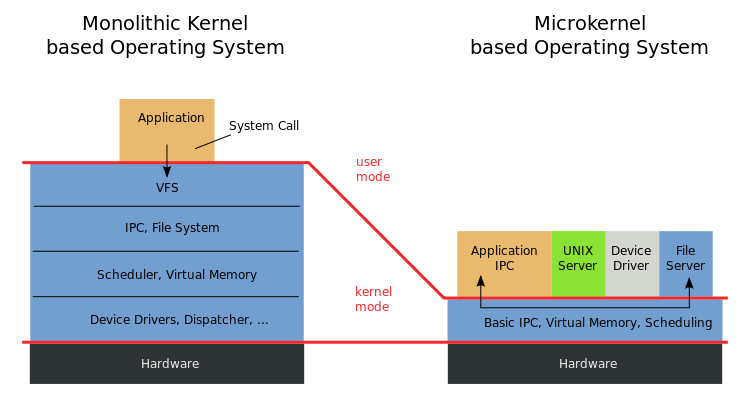
\includegraphics[scale=0.5]{images/mono-microkernel.png}
  \caption[Caption for LOF]{Overview of exo-kernel\footnotemark}
\end{figure}
\footnotetext{\url{https://en.wikipedia.org/wiki/Microkernel\#mediaviewer/File:OS-structure.svg}}

\subsection{Exokernel}
\begin{itemize}
\item Force as few abstractions as possible on developers, enabling them to make as many decisions as possible about hardware abstractions.

\item Tiny, since functionality is limited to ensuring protection and multiplexing of resources.

\item The kernel only ensures that the requested resource is free, and the application is allowed to access it.

\item Allows direct access to hardware from user space programs
\end{itemize}

\begin{figure}[H]
  \centering
  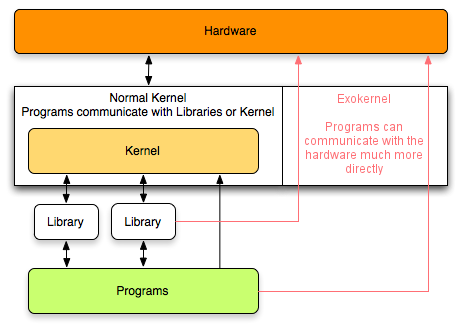
\includegraphics[scale=0.5]{images/exokernel.png}
  \caption[Caption for LOF]{Overview of exo-kernel\footnotemark}
\end{figure}
\footnotetext{\url{https://en.wikipedia.org/wiki/Exokernel\#mediaviewer/File:Exokernel\_revised(english).png}}
